\chapter{Perbedaan Docker Version}

\section{Pembuka}
Docker mulai dirilis pada tahun 2013 dimulai dari versi 0 hingga saat ini docker telah mencapai versi 20. Pada setiap update versi nya docker memberikan 
fitur baru atau perbaikan dari versi rilisan sebelumnya. Detail rilisan dapat dilihat di website dokumentasi docker 

https://docs.docker.com/engine/release-notes/. 

\begin{figure}
    Jika ingin mengecek versi docker melalui command line : 

    COMMAND: \textcolor{Blue}{docker version}

    \begin{center}
        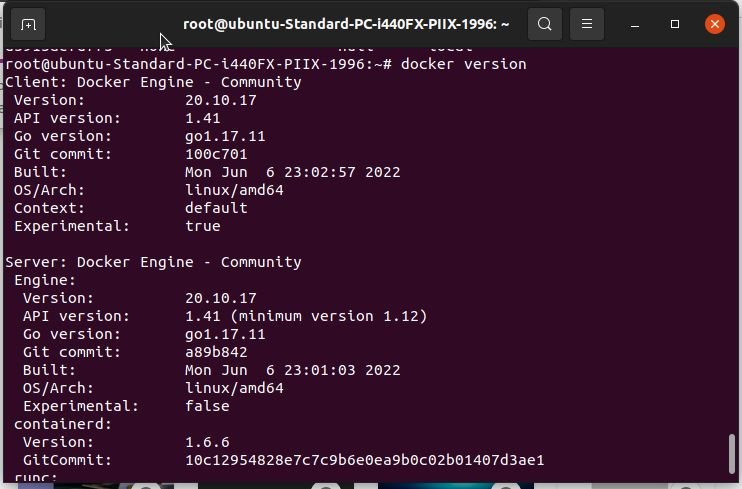
\includegraphics[width=\linewidth]{image/63.jpg}
        \caption{Cek versi docker}
        \label{fig:my_figure}
    \end{center}

    \section{Perbedaan docker version}
    Berikut perbedaan yang dari versi docker 1 - versi 20 :
\end{figure}

\begin{table}[]
\begin{tabular}{ |p{1.7cm}|p{1.6cm}|p{1.6cm}|p{1.6cm}|p{1.6cm}|p{1.6cm}|p{1.6cm}|  }
\hline
\multicolumn{1}{c}{\#}          & \multicolumn{1}{c}{Versi 1}   & \multicolumn{1}{c}{Versi 17} & \multicolumn{1}{c}{Versi 18}  & \multicolumn{1}{c}{Versi 19} & \multicolumn{1}{c}{Versi 20}  \\
\hline
Tahun Rilis & 2014-2017 & 2018     & 2018-2019 & 2021     & 2020-2022 \\
\hline
Builder     & Support for comperessing build, step number, network & Support for ADD urls without any sub path & Added prune options to the API  & Beta versions of apparmor are now parsed correctly preventing build failures         & Updated the bundled version of buildx to v0.8.0          \\
\hline
Networking  & Support attachable network, windows server 2016 overlay, sepecifying IP Address          & Support verbose info to partial overlay ID         &  Added SSH agent socket forwarder when using BuildKit         & Disable IPv6 Router Advertisements to prevent address spoofing.         &  Update libnetwork to fix publishing ports on environments with kernel boot          \\
\hline
 API  & Support secrets in docker stack deploy with compose file        &  Support for proxy configuration in config.json        &   Updated API version to 1.39        & Updated API version to v1.40.         & Update API version to v1.41          \\
\hline
Plugins     & Support global scoped network plugins, upgrade plugin      &  Make plugin removes more resilient to failure        & Configured containerd log-level to be the same as dockerd          & Added basic framework for writing and running CLI plugins         &  Socker plugin create making compatible with older versions of Docker         \\
\hline
Security    & Selinux labeling of volumes shared in a container         & Redact secret data on secret creation & Added support for build-time secrets when using BuildKit          & Prevent an invalid image from crashing docker daemon         & Profiles: seccomp: update to Linux 5.11 syscall list          \\
\hline
\end{tabular}
\end{table}